\section{Particle Dark Matter \Contact{Haibo}}
\label{sec:particles}

\Contributors{Haibo Yu, Matthew Buckley, Vera Gluscevic, Kimberly Boddy, Francis-Yan Cyr-Racine, Annika Peter, Manoj Kaplinghat, Alex Drlica-Wagner}

%\footnote{WIMPs and axions are not truly ``collisionless" because they require a coupling with other particles during their birth epoch in the early universe.  However, their interactions are so small that they are effectively collisionless particles for cosmology applications after that epoch.  Hence, WIMPs and axions are often considered to be the canonical examples of particle models for the CDM paradigm even though they are technically not completely collisionless.\AHGP{I added this.  Not sure this is the best place for it, but it would be good if this idea went somewhere.}}  

The standard \LCDM cosmological model assumes that dark matter is fully nonrelativistic and interacts purely via gravitational interactions during the process of structure formation. However, a significant dark matter thermal velocity dispersion or the presence of large non-gravitational interactions in the dark sector, such as dark matter self-interactions, couplings to other dark sector particles, or couplings to Standard Model particles, can alter the distribution of dark matter in ways that are observable with LSST. Here we focus on three representive minimal extensions to CDM -- warm dark matter (WDM), self-interacting dark matter (SIDM), and baryon-scattering dark matter (BSDM) --  to demonstrate how measurements of the distribution of dark matter can be used to constrain its micro-physical particle properties. We leave an in-depth discussion of the particle physics responsible for producing these models to the literature; however, we do attempt to connect astrophysical observables to specific terms in the interaction Lagrangian for each model.

\subsection{Warm Dark Matter (WDM)}
\label{sec:wdm}

In the standard thermal dark matter paradigm, primordial inhomogeneities in the matter density field are washed out by collisional damping and free streaming of particle dark matter \citep{Hofmann:2001,Green:2003un, Bertschinger:2006nq, Loeb:2005pm}.  
For a canonical 100-GeV thermal relic dark matter particle \citep[\eg, the WIMP;][]{Jungman:1995df}, these processes erase cosmological perturbations with $M \leq 10^{-6} \Msun$ \citep[i.e., Earth mass;][]{Green:2003un, 2005Natur.433..389D}. 
Lighter particles continue to free stream until later times, thus suppressing the formation of structure at higher mass scales (\eg, structure formation occurs bottom-up for scales larger than the free-streaming scale and top-down for scales smaller than the free-streaming scale). Because these particles are created while they are semi-relativistic, they are conventionally referred to as warm dark matter (WDM) \citep{Bond:1983hb,Bode:2000gq,Dalcanton:2000hn}. 
WDM constitutes a subclass of sub-GeV dark matter candidates.

One well-motivated WDM candidate is a sterile neutrino, $\nu_{\rm s}$, with a mass in the keV range \citep[\eg][]{Abazajian:2017tcc,Adhikari:2017}. The most relevant Lagrangian term in this case is simply the Majorana mass term,
\begin{equation}
    \mathcal{L} \supset -\frac{1}{2}M_{\rm s}\bar{\nu}_{\rm s} \nu_{\rm s}.
\end{equation}
Interestingly, such a sterile neutrino typically mixes with active Standard Model neutrinos \citep[\eg,][]{Asaka:2005an}, allowing the former to decay and leading to a potentially observable X-ray signal \citep[\eg,][]{Abazajian:2001vt}. A possible hint of such a signal has been found in deep X-ray data in the form of a narrow 3.5 keV line \citep{Boyarsky:2014, Bulbul:2014, Boyarsky:2015, Iakubovskyi:2015}, which has prompted renewed interest in understanding structure formation in WDM cosmologies \citep[\eg,][]{Lovell:2013ola,Bose:2016irl,Bozek:2018ekc}. Generally speaking, both the sterile neutrino mass and its thermal history play an important role in determining the small-scale dark matter distribution within any given particle model. For instance, at a fixed particle mass, a species created in the early universe with a velocity distribution that is skewed towards low-momentum particles \citep[\eg,][]{Shi:1998km,Venumadhav:2015pla} will display less free-streaming damping of cosmological structure than a species with a thermal (i.e., Fermi-Dirac) distribution. To avoid ambiguity, it is customary to quote WDM constraints simply in terms of a particle mass $m_{\rm WDM}$, assuming that the DM followed a thermal distribution at early times.

The free-streaming scale can be approximated by the (comoving) size of the horizon when the WDM particles become nonrelativistic.
%The comoving horizon size at $z = 10^7$ corresponds to $m = 2.5 \keV$, and is approximately $50 \kpc$, which is significantly smaller than the scale derived above for $\Lstar$ galaxies \citep{Adhikari:2017}
Astrophysical constraints on WDM are generally placed by observing the smallest gravitationally bound dark matter halos.  
In particular, the half-mode mass (the scale at which the dark matter transfer function is reduced by half) represents a characteristic halo mass scale below which halo abundances are suppressed sufficiently to yield observable consequences. 
The half-mode halo mass, \Mhm, is related to the WDM thermal relic particle mass, \mWDM, by \citep[\eg][]{schneider2012,Bullock:2017xww}
\begin{equation} \label{eqn:Mhm}
    M_{\rm hm} = 5.5 \times 10^{10} \left( \frac{m_{\rm WDM}}{1 {\rm keV}} \right)^{-3.33} \Msun.
\end{equation}
Thus, an observed suppression in the abundance of dark matter halos smaller than \Mhm could signify the existence of a thermal dark matter particle with mass
\begin{equation} \label{eqn:mWDM}
    m_{\rm WDM} =  3.33 \left(\frac{M_{hm}}{10^{9} {\rm M_\odot}} \right)^{-0.3} \keV.
\end{equation}
It is important to remember that $m_{\rm WDM}$ is the thermal-relic-equivalent particle mass. Translating measurements of the halo mass function to constraints on the particle mass for a specific WDM model depends on the specific mapping between particle mass and the early-time momentum distribution.

Measurements of the Lyman-$\alpha$ forest \citep[\eg][]{Viel:2013,2017PhRvD..96b3522I} and ultra-faint satellite galaxies \citep[\eg][]{Jethwa:2018,Kim:2017iwr} place lower bounds on the mass of thermally produced WDM particles at $\roughly 3$--$5\keV$, corresponding to a halo mass scale of $\roughly 10^8-10^9 \Msun$.
The sensitivity and wide-area coverage of LSST has the potential to extend measurements of the dark matter halo mass function by three orders of magnitude, down to $\roughly 10^6 \Msun$ (\secref{halo_mass}). 
These observations have the potential to constrain WDM particle masses \CHECK{$m_{\rm WDM} \gtrsim 18\keV$}, thus effectively testing putative signatures of keV-mass sterile neutrinos.


\subsection{Self-Interacting Dark Matter (SIDM)}
%\Contributors{Haibo, Francis-Yan, Manoj?,...}
\label{sec:sidm}

The self-interacting dark matter (SIDM) paradigm posits additional interactions in the dark sector \citep[\eg,][]{1992ApJ...398...43C,Spergel:1999mh,Dave:2000ar,Firmani:2000ce}, which allow energy and momentum exchange between particles within dark matter halos \citep[see][for a recent review]{Tulin:2017ara}. The figure of merit for dark matter halo structure is the cross section per dark matter particle mass, $\sigma/m_\chi$.
%where $\sigma$ is a transfer cross-section,
%\begin{equation}
%    \sigma = \int d\Omega (1-\cos\theta) \frac{d\sigma}{d\Omega}.
%\end{equation}
%\AHGP{For identical particles, isn't this the wrong cross section?  Kim Boddy and Hai-Bo Yu advocate for the viscosity cross section.}
Dark matter self-interactions with cross sections per mass roughly equivalent to the strong nuclear force ($\sigma/m_\chi \sim 1 \cmg$) would imply ${\cal O}(1)$ energy exchange in the central regions of halos within the age of the universe \citep{2012MNRAS.423.3740V,2013MNRAS.431L..20Z,2013MNRAS.430..105P,Rocha:2012jg}. This  would thermalize the inner regions of dark matter halos --- where visible baryonic matter resides --- with observational consequences \citep[\eg][]{Kaplinghat:2013xca}. For low-surface brightness galaxies, SIDM thermalization leads to a cored inner density profile, in contrast to the cupsy profiles predicted in CDM. For high-surface brightness galaxies, thermalization leads to a small core and more concentrated SIDM distribution because of the presence of the baryonic potential \citep{Kaplinghat:2015aga}. It has been shown that SIDM can explain both the diversity and uniformity of galaxy rotation curves, for $\sigma/m_\chi \gtrsim 1\cmg$ on galaxy scales \citep{Kamada:2016euw,Creasey:2016jaq,Ren:2018jpt}. This diversity of properties within SIDM halos also extends to galaxy cluster scales \citep{Robertson:2017mgj}.

%\ADW{This is coming from Section VI.C in 1705.02358.}
Large self-interaction cross sections are required to modify galactic structure, and such cross sections suggest either strongly-coupled systems \citep[\eg,][]{Frandsen:2011kt,Hochberg:2014dra,Hochberg:2014kqa} or a light mediator with perturbative couplings \citep[\eg,][]{Feng:2009mn,Ackerman:2008gi,Kaplan:2009de,Feng:2009hw,Buckley:2009in,Loeb:2010gj,Tulin:2012wi,Tulin:2013teo,Schutz:2014nka,Blennow:2016gde}. An interesting example of the latter type of model would be to charge dark matter under a $U(1)$ gauge symmetry. %which may be either broken or unbroken. 
Exchange of the gauge boson (a ``dark photon'') then mediates self-interactions, analogous to Rutherford scattering. A phenomenologically similar model replaces the vector mediator with a light scalar. The interaction Lagrangian is then described by %\citep{1210.0900,1302.3898}:
\begin{equation}
\label{eq:sidm}
{\cal L_{\rm int}}=\bigg\{
\begin{array}{c l}
g_\chi\bar{\chi}\gamma^\mu\chi\phi_\mu & \text{(vector mediator)}\\
g_\chi\bar{\chi}\chi\phi & \text{(scalar mediator)} \, ,
\end{array}
\end{equation}
where $\chi$ is the dark matter particle (which we assume to be a fermion for concreteness), $\phi$ is the mediator, and $g_\chi$ is the coupling constant. In the non-relativistic limit, self-interactions are described by the Yukawa potential
\begin{equation}
V(r)=\pm\frac{\alpha_\chi}{r}e^{-m_\phi r},
\label{eq:yukawa}
\end{equation}
where $\alpha_\chi = g_\chi^2/4\pi$. In order for annihilation through the mediator to not deplete the dark matter relic abundance during the early universe, it may be necessary to assume asymmetric dark matter (that is, dark matter which is composed mainly of $\chi$, with a minimal admixture of $\bar\chi$). In that case, the vector mediator would provide only a repulsive potential (``$+$'' in Eq.~\ref{eq:yukawa}), while the scalar mediator would have an attractive potential (``$-$'').

%(a $+$ in Eq.~\eqref{eq:yukawa}) (a $-$ sign)

In these light mediator models, the self-scattering cross section generally depends on the relative velocity of colliding dark matter particles, $v_{\rm rel}$, and scattering is not isotropic. In practice, we often consider the transfer (viscosity) cross section, defined as $\sigma_T = \int d\Omega(1-\cos\theta)d\sigma/d\Omega$ ($\sigma_V = \int d\Omega\sin^2\theta d\sigma/d\Omega$), to regulate small-angle scatterings and use them as a proxy to match to SIDM N-body simulations with a constant cross section for a given halo-mass scale \citep[][]{Tulin:2013teo,Kahlhoefer:2013dca}. The overall feature of the velocity dependence predicted in the models can be summarized as follows. When the momentum transfer is much larger than the mediator mass, the scattering is in the Rutherford limit, i.e., $\sigma/m_\chi\propto v^{-4}_{\rm rel}$. While in the opposite limit, $m_\chi v_{\rm rel}\ll m_\phi$, $\sigma/m_\chi$ is nearly a constant. If the scattering is in the quantum resonant regime for $\chi\textup{-}\bar{\chi}$ collisions, $m_\chi v_{\rm rel}\sim m_\phi$, $\sigma/m_\chi\propto v^{-2}_{\rm rel}$. Since large dark matter halos have much larger dark matter velocities compared to smaller halos, observations from different scales, ranging from dwarf galaxies to galaxy clusters, provide important tests of these models.

%($m_\chi$, $m_\phi$, $\alpha_\chi$)

There are numerous observations that are sensitive to dark matter self scattering \citep[\eg,  Table 1 in][]{Tulin:2017ara}. Notably, merging galaxy clusters, such as the Bullet cluster  \citep{Randall:2007ph,2017MNRAS.465..569R}, have been used to put an upper bound on the self-interaction cross section at large particle velocities \citep[\eg,][]{Kahlhoefer:2013dca,Kahlhoefer:2015vua,Kim:2016ujt,Harvey:2016bqd,Robertson:2016qef,Wittman:2017gxn}, yielding $\sigma/m_\chi \lesssim 2 \cmg$ for $v_{\rm rel} \sim 1000\textup{--}4000 \kms$. Moreover, observations from well-relaxed galaxy clusters \citep{Newman++11,Newman:2013,Newman++13b} show $\sigma/m_\chi \sim 0.1 \cmg$ for $v_{\rm rel} \sim 1500 \kms$ to be consistent with their inferred core sizes~\citep{Kaplinghat:2015aga,Andrade:2019wzn}. The diversity of rotation curves observed in spiral galaxies can be explained by dark matter scattering with $\sigma/m_\chi \gtrsim 1 \cmg$ in the range of $v_{\rm rel}\sim50\textup{--}200 \kms$. For these spiral galaxies, the large cross section is driven by galaxies with a high density core. In contrast, high surface brightness galaxies are baryon-dominated in their central regions and are thus effectively insensitive to the value of $\sigma/m_\chi$ \citep{Kamada:2016euw,Ren:2018jpt}. 

Velocity-dependent SIDM models with $\sigma/m_\chi \gtrsim 1 \cmg$ in dwarf galaxies and $\sigma/m_\chi \sim 0.1 \cmg$ in galaxy clusters are able to fit existing observational data (\figref{sidm_sigma}). This result has important implications for the particle properties of SIDM. For instance, consider the dark photon model given in Eq.~(\ref{eq:sidm}) and assume $\alpha_\chi=1/137$ to match the fine structure constant in the visible sector, we can determine $m_\chi\approx 15 \GeV$ and $m_\phi \approx 17 \MeV$ \citep{Kaplinghat:2015aga} and even infer the production mechanism of SIDM in the early universe \citep{Huo:2017vef}. Since LSST will probe scales ranging from the largest galaxy clusters to the smallest dwarf galaxy, it will be able to detect the influence of scattering cross sections at the level of $\sigma/m_\chi \sim 0.1$--$1 \cmg$ over a wide range of velocities. Thus, LSST will significantly improve our understanding of the self-interacting nature of dark matter. 

\begin{figure}
\centering
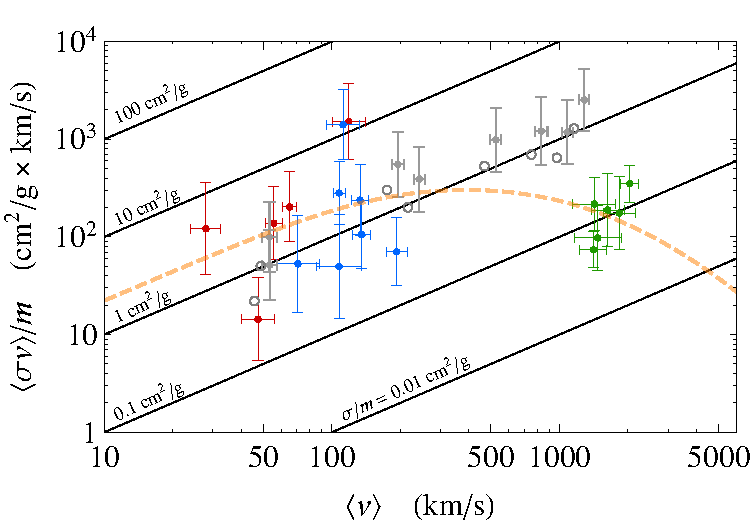
\includegraphics[width=0.6\columnwidth]{figures/sigmav.pdf}
\caption{Velocity-weighted self-interaction cross section per unit mass as a function of average relative particle velocity in a halo. Data points from astrophysical observations correspond to dwarf galaxies (red), low-surface-brightness galaxies (blue), and galaxy clusters (green). 
Diagonal lines show constant values of $\sigma/m_\chi$. 
Gray points are fits to mock data from SIDM simulations, with fixed $\sigma/m_\chi = 1 \cmg$.
Figure taken from \citet{Kaplinghat:2015aga}.
}
\label{fig:sidm_sigma}
\end{figure}

It is also natural to expect that SIDM has a modified matter power spectrum compared to CDM. For instance, in SIDM models where the dark matter particle couples to a massless particle in the early universe, either directly or through a light mediator, the tight coupling between dark matter and dark radiation can lead to dark acoustic oscillations \citep{Cyr-Racine:2013ab,Cyr-Racine:2013fsa}, resulting in a suppressed and oscillatory power spectrum \citep[\eg][]{1992ApJ...398...43C,Boehm:2001hm,Boehm:2004th,Feng:2009mn,Aarssen:2012fx}. It has been shown that realistic realizations of SIDM strongly prefer such a scenario \citep{ Huo:2017vef}.

To see the reach of LSST on the SIDM damping effect, we estimate the cut-off scale on the field halo mass due to the dark acoustic oscillations as $M_{\rm cut}\approx0.7\times10^{8}({\rm keV/T_{\rm kd}})^3 \Msun$~\citep{1512.05349}, where $T_{\rm kd}$ is the kinetic decoupling temperature. For SIDM models, where a dark matter particle ($\chi$) couples to a massless fermion ($f$) via a light mediator ($\phi$), $T_{\rm kd}$ is given by~\citep{Aarssen:2012fx,Cyr-Racine:2015ihg}
\begin{equation}
T_{\rm kd}\approx\frac{1.38~{\rm keV}}{\sqrt{g_\chi g_f}}\left(\frac{m_\chi}{100 \GeV}\right)^{\frac{1}{4}}\left(\frac{m_\phi}{10 \MeV}\right)\left(\frac{g_\star}{3.38}\right)^{\frac{1}{8}}\left(\frac{0.5}{\xi}\right)^{\frac{3}{2}},
\label{eq:tkd}
\end{equation}
where $g_f$ is the $\xi\textup{--}f$ coupling constant, $g_\star$ the is the number of massless degrees of freedom at decoupling and $\xi$ parameterizes the ratio of dark-to-visible temperatures. \citet{Huo:2017vef} recasts the Lyman-$\alpha$ bound on WDM to set upper limit on the decoupling temperature $T_{\rm kd}\gtrsim 1 \keV$, corresponding to the minimal halo mass $\roughly 10^8 \Msun$. Since LSST has the potential to extend measurements of the dark matter halo mass function by three orders of magnitude (\secref{halo_mass}), the expected sensitivity on the decoupling temperature is $T_{\rm kd}\sim 10 \keV$. If LSST detects a cutoff on the halo mass function, we can determine the corresponding $T_{\rm kd}$ and further narrow down the particle parameters contained in the Lagrangian via Eq.~(\ref{eq:tkd}) after combining with the measurements of $\sigma/m_\chi$ discussed above. Moreover, since the damping effect can also suppress the number of subhalos in the Milky Way, we expect LSST to provide another constraint on $T_{\rm kd}$ by providing a more complete census of ultra-faint satellites. In addition, although the acoustic damping effect may look similar to the free-streaming one \citep[\eg][]{1512.05349}, distinct signatures can be imprinted on the halo mass function \citep{Buckley:2014ab,Sameie:2018juk} or the Lyman-$\alpha$ forest spectrum \citep{Krall:2017xcw,Bose:2018juc}. By combining observables, including those from LSST, it might thus be possible to distinguish between WDM and SIDM with a damped matter power spectrum due to early-universe interactions (\secref{combine_probes}).

     
\subsection{Baryon-Scattering Dark Matter (BSDM) \Contact{Vera}}
%\Contributors{Vera, Kim, ...}
\label{sec:bsdm}

In the standard WIMP scenario, dark matter may be directly observable through its scattering with Standard Model particles.
These models are conventionally probed by direct detection experiments that search for scattering between dark matter particles (from the local Galactic halo) and nuclei in their detectors.
These experiments are placed deep underground to provide shielding from cosmic-ray backgrounds and achieve exquisite sensitivity for low scattering cross sections. 
These experiments are largely insensitive to dark matter with very large scattering cross section because such particles would scatter many times before reaching the experiment, thus losing most of their kinetic energy \citep[\eg][]{Zaharijas:2004jv}.
%However, given the current null results from these experiments, 
Thus, it is important to broadly explore parameter space outside the standard WIMP region of interest.

Cosmological and astrophysical observables are unique and complementary probes of baryon-scattering dark matter (BSDM) models.
In particular, they are sensitive to very large (closer to nuclear-scale rather than weak-scale) scattering cross sections and sub-GeV dark matter masses, both of which are inaccessible to direct searches.
Such large cross sections may arise in a number of models.
One such model posits that dark matter is a flavor singlet sexaquark composed of $uuddss$ quarks \citep{Farrar:2017eqq}.
In this case, the scattering cross section with nucleons is expected to be geometric, though velocity-dependent enhancements may exist at very low energies, depending on the form of the sexaquark-nucleon potential.
For the sexaquark to be a viable dark matter candidate, it must be stable or have a sufficiently long lifetime; this criterion sets the sexaquark mass to be below a few GeV.
Alternatively, dark matter may be charged under a dark version of electromagnetism with field strength $\tilde{F}_{\mu\nu}$, which may kinetically mix with ordinary electromagnetism~\citep{Holdom:1985ag}:
\begin{equation}
    \mathcal{L} \supset \frac{\kappa}{2} F^{\mu\nu} \tilde{F}_{\mu\nu} ,
\end{equation}
where $\kappa$ parameterizes the strength of the mixing.
In this scenario, dark matter acquires a fractional amount of electric charge (proportional to $\kappa$ and its dark charge), allowing it to scatter with electrons and protons via Coulomb interactions that have a velocity dependence of $v^{-4}$.
This interaction is significant at late cosmological times, as the universe expands and the momentum of matter redshifts away.

Instead of focusing on particular theories, it is possible to describe the low-energy scattering processes of BSDM models with a nonrelativistic effective field theory~\citep{Fan:2010gt,Fitzpatrick:2012ix,Anand:2013yka}.
The effective Lagrangian has the form
\begin{equation}
    \mathcal{L}_\textrm{eff}(\vec{x})
    = c \Psi_\chi^\ast (\vec{x}) \mathcal{O}_\chi \Psi_\chi (\vec{x})
    \Psi_N^\ast (\vec{x}) \mathcal{O}_N \Psi_N (\vec{x}) ,
\end{equation}
where $\Psi (\vec{x})$ are the nonrelativistic fields for the dark matter, $\chi$, and nucleon, $N$.
Dark matter experiments seek to constrain and measure the coefficient $c$ for a variety of possible operators $\mathcal{O}_\chi$ and $\mathcal{O}_N$ that encode the BSDM physics.
However, regardless of the specific underlying BSDM model, cosmological observables are sensitive only to the magnitude (which scales as $c^2$) and velocity dependence of the cross section.
Thus, while laboratory searches for dark matter typically rely on assumptions about the detailed form of the interaction, cosmology offers very broad and generic probes of dark matter physics.

In a cosmological setting, scattering results in the exchange of momentum between the dark matter and the baryon fluids.
The momentum transfer induces a drag force, which suppresses structure increasingly at smaller scales. 
The effect of scattering is qualitatively similar to a cutoff in the matter power spectrum arising in the WDM and SIDM scenarios (\figref{dmbaryon_pk}).
This feature can be sought with tracers of matter on all observable scales. 
The best cosmological and astrophysical limits so far come from CMB temperature, polarization, and lensing anisotropy measurements~\citep{Xu:2018efh,Boddy:2018kfv,Gluscevic:2017ywp,Boddy:2018wzy,Slatyer:2018aqg}, cosmic-ray observations \citep{Cappiello:2018hsu}, and Lyman-$\alpha$-forest measurements~\citep{Dvorkin:2013cea,Xu:2018efh}. 
LSST will probe the matter power spectrum on even smaller scales, through substructure measurements from dwarf galaxies in the Local Volume, gaps in stellar streams, galaxy strong lensing, and galaxy-galaxy weak lensing; such observations will substantially extend current experimental sensitivity to BSDM models.

\begin{figure}
\centering
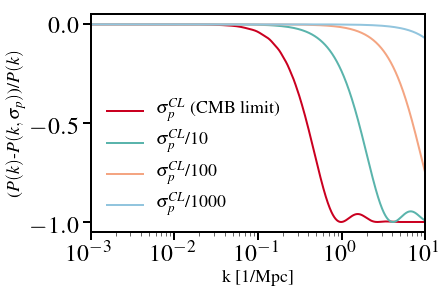
\includegraphics[width=0.6\columnwidth]{figures/dmbaryon_pk2.png}
\caption{Residuals in the linear matter power spectrum between the CDM case and a case where dark matter has a velocity-independent, spin-independent scattering with protons. The dark matter particle mass is set to $1\MeV$, and all other cosmological parameters are set to their best-fit Planck 2015 values \citep{Ade:2015xua}. Different residual curves display cutoffs at different angular scales, controlled by the magnitude of the interaction cross section. The highest cross section shown corresponds to the current 95\% confidence-level upper limit inferred from analyses of CMB data \citep{Gluscevic:2017ywp,Boddy:2018kfv}.
}
\label{fig:dmbaryon_pk}
\end{figure}

As an example, a measurement of the minimum halo mass translates into an upper limit on the dark matter-proton interaction cross section, based on the corresponding cutoff in the matter power spectrum $P(k)$. \figref{dmbaryon_pk} shows how the position of the cutoff in the linear $P(k)$ varies as a function of the interaction cross section. For example, a lower limit on the cutoff of $k_\text{cutoff} \sim 10/\Mpc$ roughly corresponds to an upper limit on the cross section which is 100 times more stringent than the current limit from CMB searches. Using limits on WDM as a proxy for a suppressed $P(k)$, a minimum halo mass of $\roughly 10^6 \Msun$ would imply an improvement of roughly five orders of magnitude compared to the best current cosmological limits on the interaction cross section.
